\documentclass[mathserif,compress]{beamer} 
\usepackage{pdfpages}
%\usepackage{handoutWithNotes} 
%\pgfpagesuselayout{4 on 1 with notes}[a4paper, border shrink=5mm]
%\pgfpageslogicalpageoptions{1}{border code=\pgfusepath{stroke}}
%\pgfpageslogicalpageoptions{2}{border code=\pgfusepath{stroke}}
%\pgfpageslogicalpageoptions{3}{border code=\pgfusepath{stroke}}
%\pgfpageslogicalpageoptions{4}{border code=\pgfusepath{stroke}}

\usepackage{beamerthemeDresden} 
\usepackage[english]{babel}
\usepackage{amsmath,amssymb}
\usepackage[latin1]{inputenc}
\usepackage{palatino}
\usepackage{graphicx}
\usepackage{subfigure}
\usepackage{pgf}
\usepackage{relsize}
\usepackage{tabularx}
\usepackage{setspace}
%\beamertemplateshadingbackground{red!1}{blue!1}
% Use some nice templates
\beamertemplatetransparentcovereddynamic  


\def\beq{\begin{equation}}
\def\eeq{\end{equation}}
\def\bit{\begin{itemize}}
\def\eit{\end{itemize}}
\def\bdm{\begin{displaymath}}
\def\edm{\end{displaymath}}
\def\ben{\begin{enumerate}}
\def\een{\end{enumerate}}
\def\bc{\mathbf{c}}
\def\be{\mathbf{e}}
\def\bh{\mathbf{h}}
\def\bn{\mathbf{n}}
\def\br{\mathbf{r}}
\def\bs{\mathbf{s}}
\def\bu{\mathbf{u}}
\def\bw{\mathbf{w}}
\def\bx{\mathbf{x}}
\def\by{\mathbf{y}}
\def\bz{\mathbf{z}}
\def\bA{\mathbf{A}}
\def\bB{\mathbf{B}}
\def\bC{\mathbf{C}}
\def\bD{\mathbf{D}}
\def\bG{\mathbf{G}}
\def\bI{\mathbf{I}}
\def\bM{\mathbf{M}}
\def\bP{\mathbf{P}}
\def\bQ{\mathbf{Q}}
\def\bR{\mathbf{R}}
\def\bS{\mathbf{S}}
\def\bV{\mathbf{V}}
\def\bW{\mathbf{W}}
\def\bX{\mathbf{X}}
\def\bY{\mathbf{Y}}
\def\bZ{\mathbf{Z}}
\def\cB{\mathcal{B}}
\def\cF{\mathcal{F}}
\def\cI{\mathcal{I}}
\def\cK{\mathcal{K}}
\def\cU{\mathcal{U}}
\def\balpha{\mbox{\boldmath $\alpha$}}
\def\bbeta{\mbox{\boldmath $\beta$}}
\def\bepsilon{\mbox{\boldmath $\epsilon$}}
\def\bdelta{\mbox{\boldmath $\delta$}}
\def\bgamma{\mbox{\boldmath $\gamma$}}
\def\bldeta{\mbox{\boldmath $\eta$}}
\def\bphi{\mbox{\boldmath $\phi$}}
\def\bkappa{\mbox{\boldmath $\kappa$}}
\def\blambda{\mbox{\boldmath $\lambda$}}
\def\bmu{\mbox{\boldmath $\mu$}}
\def\bnu{\mbox{\boldmath $\nu$}}
\def\btheta{\mbox{\boldmath $\theta$}}
\def\brho{\mbox{\boldmath $\rho$}}
\def\bDelta{\mbox{\boldmath $\Delta$}}
\def\bLambda{\mbox{\boldmath $\Lambda$}}
\def\bSigma{\mbox{\boldmath $\Sigma$}}
\def\var{\textrm{var}}
\def\cov{\textrm{cov}}
\def\log{\textrm{log}}
\def\median{\textrm{median}}
\def\argmin{\textrm{arg min }}
\def\bzero{\mathbf{0}}
\def\bone{\mathbf{1}}
\def\Poi{\textrm{Poi}}
\def\Unif{\textrm{Unif}}
\def\upp{^{\prime}}
\def\upi{^{-1}}
\newcommand{\cye}[1]{\color{yellow!70!black}#1}
\newcommand{\cre}[1]{\color{red!70!black}#1}
\newcommand{\cbl}[1]{\color{blue!70!black}#1}
\newcommand{\cgr}[1]{\color{green!70!black}#1}
\newcommand{\cpu}[1]{\color{blue!65!red}#1}
\newcommand{\fsz}[1]{{\footnotesize #1}}
\newcommand{\ssz}[1]{{\scriptsize #1}}

%-------------------------------------------------------------------------------

\title[]{A Quick and Dirty Bayesian Leslie Matrix Model of Norway HarpEast Data }

\author[Jay M. Ver Hoef]{Jay Ver Hoef} 

\institute[Marine Mammal Laboratory]
{
	\normalsize Marine Mammal Laboratory \\
	NOAA Fisheries Alaska Science Center \\
	Seattle, Washington and Fairbanks, Alaska, USA\\
	\vspace{0.1cm}
}
\date[11/06/20]{}
%-------------------------------------------------------------------------------
\begin{document}

%-------------------------------------------------------------------------------
\frame{\titlepage}
%-------------------------------------------------------------------------------

%-----------------------------------------------------------------------
%           The Model
%-----------------------------------------------------------------------
\begin{frame} 
\vspace{-.5cm}

Population Values 

\vspace{.2cm}
$A_{t} = \textrm{Number of Nonpups in year } t$ \\
$H^{A}_{t} = \textrm{Harvest of Nonpups in year } t$ \\
$P_{t} = \textrm{Number of Pups in year } t$ \\
$H^{P}_{t} = \textrm{Harvest of Pups in year } t$ \\
$N_{t} = A_{t} + P_{t}$ \\

\end{frame}


%-----------------------------------------------------------------------
%           The Model
%-----------------------------------------------------------------------
\begin{frame} 
\vspace{-.5cm}
A Simple Two-age Leslie Matrix Model

\vspace{.2cm}

{\tiny 
\begin{singlespace}
 Boveng, P.L., Ver Hoef, J.M., Withrow, D.E., and London, J.M. 2018. A Bayesian Analysis of Abundance, Trend and Population Viability for Harbor Seals in Iliamna Lake, Alaska. Risk Analysis 38(9): 1988-209 DOI:10.1111/risa.12988
\end{singlespace}
}

$$
  \begin{tabular}{l}
    $A_t = \delta_{t-1}(A_{t-1}-H^{A}_{t-1}) + \kappa_{t-1}(P_{t-1} - H^{P}_{t-1})$, \\
		$P_t = c_{t-1}\phi_{t-1}(A_{t-1}-H^{A}_{t-1})$,
  \end{tabular}
$$

$$
  \bn_t = \left(\begin{array}{c}
    P_t \\
    A_t \\
  \end{array}\right), \
  \bh_t = \left(\begin{array}{c}
    H^{A}_t \\
    H^{P}_t \\
  \end{array}\right), \
  \bM_t = \left( \begin{array}{ll}
      0 & c_t\phi_t \\
      \kappa_t & \delta_t
  \end{array} \right)
$$

$$
\bn_{t} = \left(\bn_{t-1} - \bh_{t-1}\right) \bM_{t-1}
$$
$c_{t} = \exp(-\rho N_{t}/1000)$ 
$c_{t} = \textrm{Exponential decay in fecundity with increased } N_{t}$ 

\end{frame}

%-----------------------------------------------------------------------
%           Priors
%-----------------------------------------------------------------------
\begin{frame} 
Parameters

$P_{1}:\textrm{ Abundance of Pups in Year }t = 1$
$A_{1}:\textrm{ Abundance of Nonpups in Year }t = 1$
$\delta_{t}:\textrm{ Adult Mortality Rate in Year }t$
$\kappa_{t}:\textrm{ Pup Mortality Rate, from Survey to Survey, in Year }t$
$\phi_{t}:\textrm{ Fecundity Rate for all Adults, to Survey Time, in Year }t$
$\rho:\textrm{ Controls Exponential Decay in Fecundity as Population }\uparrow$

Priors

$[P_{1}] = \pi(P_{1}) \sim \textrm{N}(\textrm{300,000}, \hspace{.2cm} \textrm{50,000}^{2})$ \\
$[A_{1}] = \pi(A_{1}) \sim \textrm{N}(\textrm{1,000,000}, \hspace{.2cm} \textrm{100,000}^{2})$
$[\bdelta] = \pi(\textrm{logit}(\delta_{t})) \sim \textrm{N}(2.2, 0.5^{2}) \ \forall \ t; \ \textrm{logit}^{-1}(2.2) = 0.90$
$[\bkappa] = \pi(\textrm{logit}(\kappa_{t})) \sim \textrm{N}(1.4, 0.5^{2}) \ \forall \ t; \ \textrm{logit}^{-1}(1.4) = 0.80$
$[\bphi] = \pi(\textrm{logit}(\phi_{t})) \sim \textrm{N}(-0.4, 0.5^{2}) \ \forall \ t; \textrm{logit}^{-1}(-0.4) = 0.40$
$[\rho] = \pi(\textrm{log}(\rho)) \sim \textrm{N}(-4.0, 0.5^{2})$ \\


\end{frame}

%-----------------------------------------------------------------------
%           Data and Likelihood
%-----------------------------------------------------------------------
\begin{frame} 
Data

\vspace{.2cm}
$H^{A}_t \textrm{ and } H^{P}_t \textrm{ for all years}$
$p_{t} \textrm{ an estimate of pup abundance in year }t \in \mathcal{S}$
$s_{t} \textrm{ a standard error of pup abundance in year }t \in \mathcal{S}$
$\mathcal{S} \textrm{ is an index set of sampled years from }T\textrm{ total years}$
$\mathcal{T} \textrm{ is the index set of years } t = 1,\ldots,T$
\vspace{.2cm}

Likelihood
\begin{center}
$[p_{t} \mid P_{t}, s_{t},\bdelta,\bkappa,\bphi,\rho,P_{1},A_{1},\{\bh_{t}; t \in \mathcal{T}\}] \sim \textrm{N}(P_{t},s_{t})$ \\
\end{center}
$\textrm{where } P_{t} \textrm{ is obtained from}$
\begin{center}
$\bn_{t} = \left(\bn_{t-1} - \bh_{t-1}\right) \bM_{t-1}; \ t \in \mathcal{T}$
\end{center}
$\textrm{where }\{\bn_{t}; t \in \mathcal{T}\}\textrm{ depends on }\bdelta,\bkappa,\bphi,\rho,P_{1},A_{1}$


\end{frame}

%-----------------------------------------------------------------------
%           Posteriors and MCMC Sampling
%-----------------------------------------------------------------------
\begin{frame} 

Posterior
\begin{center}
$[P_{1},A_{1},\bdelta,\bkappa,\bphi,\rho \mid \{(p_{t},s_{t}); t \in \mathcal{S}\},\{\bh_{t}; t \in \mathcal{T}\}] \propto$ \\
$\prod_{\mathcal{S}}[p_{t} \mid P_{t}, s_{t},\bdelta,\bkappa,\bphi,\rho,P_{1},A_{1},\{\bh_{t}; t \in \mathcal{T}\}][P_{1}][A_{1}][\bdelta][\bkappa][\bphi][\rho]${}
\end{center}

Posterior of $\{\bn_{t}; t \in \mathcal{T}\}$ is constructed from posteriors of $P_{1},A_{1},\bdelta,\bkappa,\bphi$ and $\rho$. 

\vspace{.2cm}
Use MCMC with Metropolis sampling to obtain sample from posterior distribution.

\vspace{.2cm}
Custom code written in R, uses batch sampling for $\bdelta,\bkappa,\bphi$, with a burnin of 10,000 samples, followed by 100,000 where only each 100$th$ sample was saved, yielding 1,000 samples from posterior. 
\end{frame}


%-----------------------------------------------------------------------
%           Trajectory Results
%-----------------------------------------------------------------------


\begin{frame} 

\begin{center}
	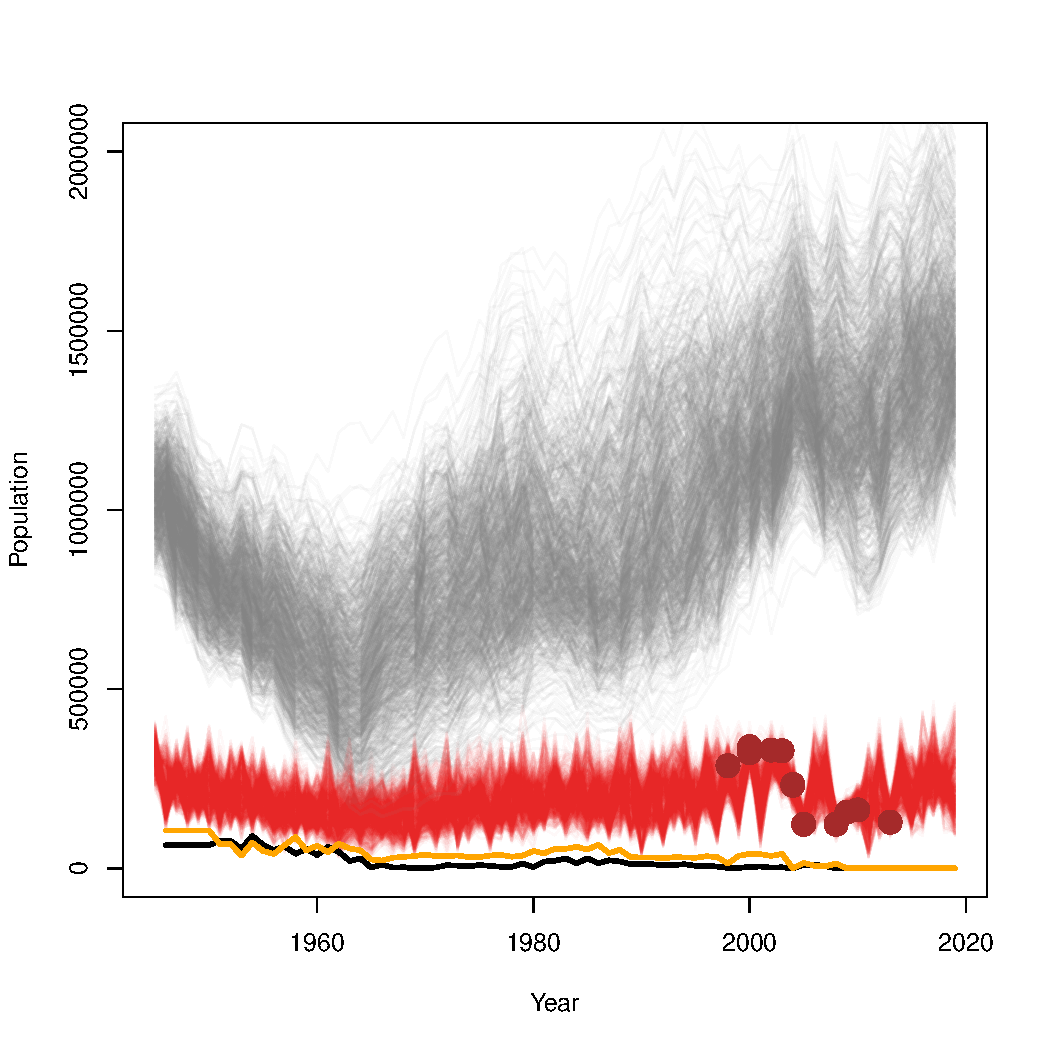
\includegraphics[height=7cm]{figure/Pop_traj} 
\end{center}
\end{frame}

%-----------------------------------------------------------------------
%           Posterior phi
%-----------------------------------------------------------------------

\begin{frame} 

\begin{center}
	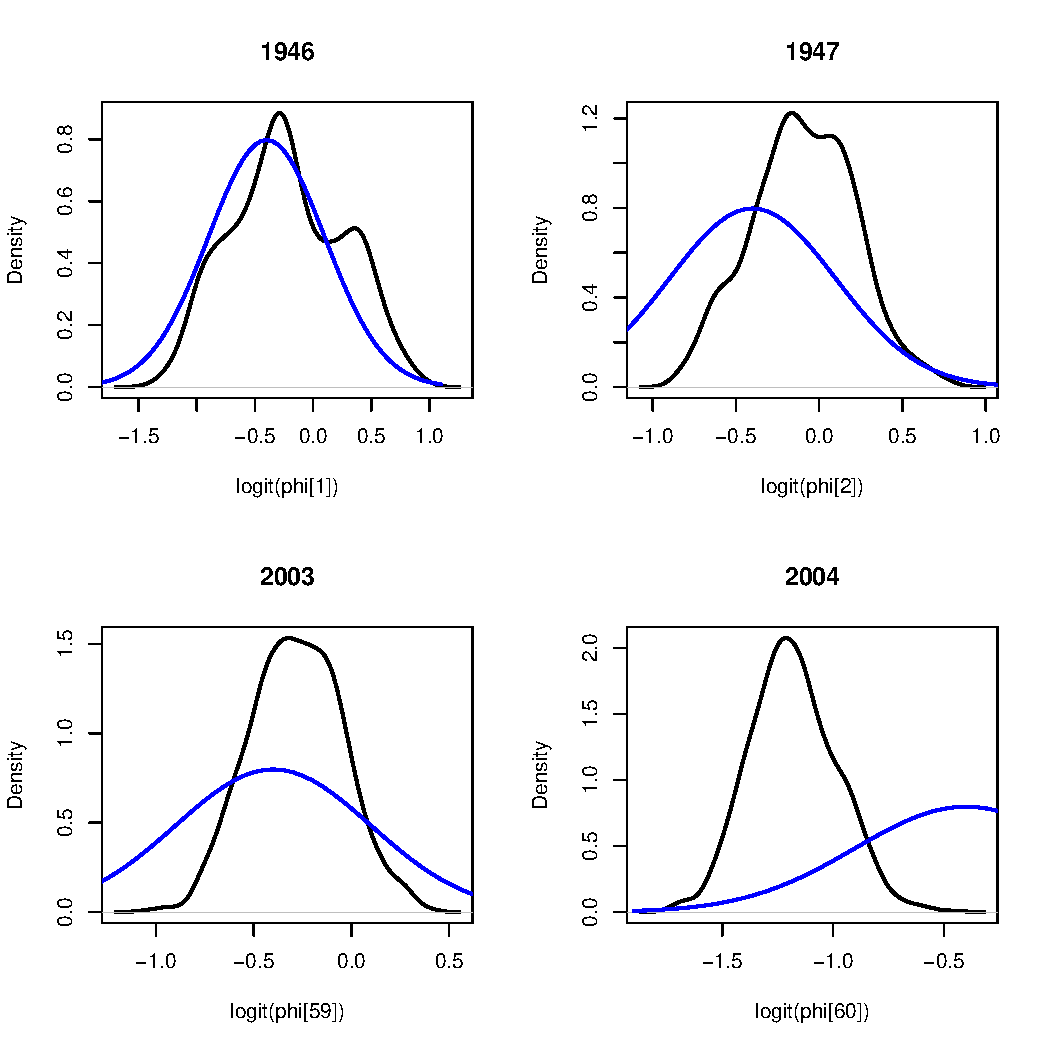
\includegraphics[height=7cm]{figure/Post_phi} 
\end{center}
\end{frame}

%-----------------------------------------------------------------------
%           Posterior delta
%-----------------------------------------------------------------------

\begin{frame} 

\begin{center}
	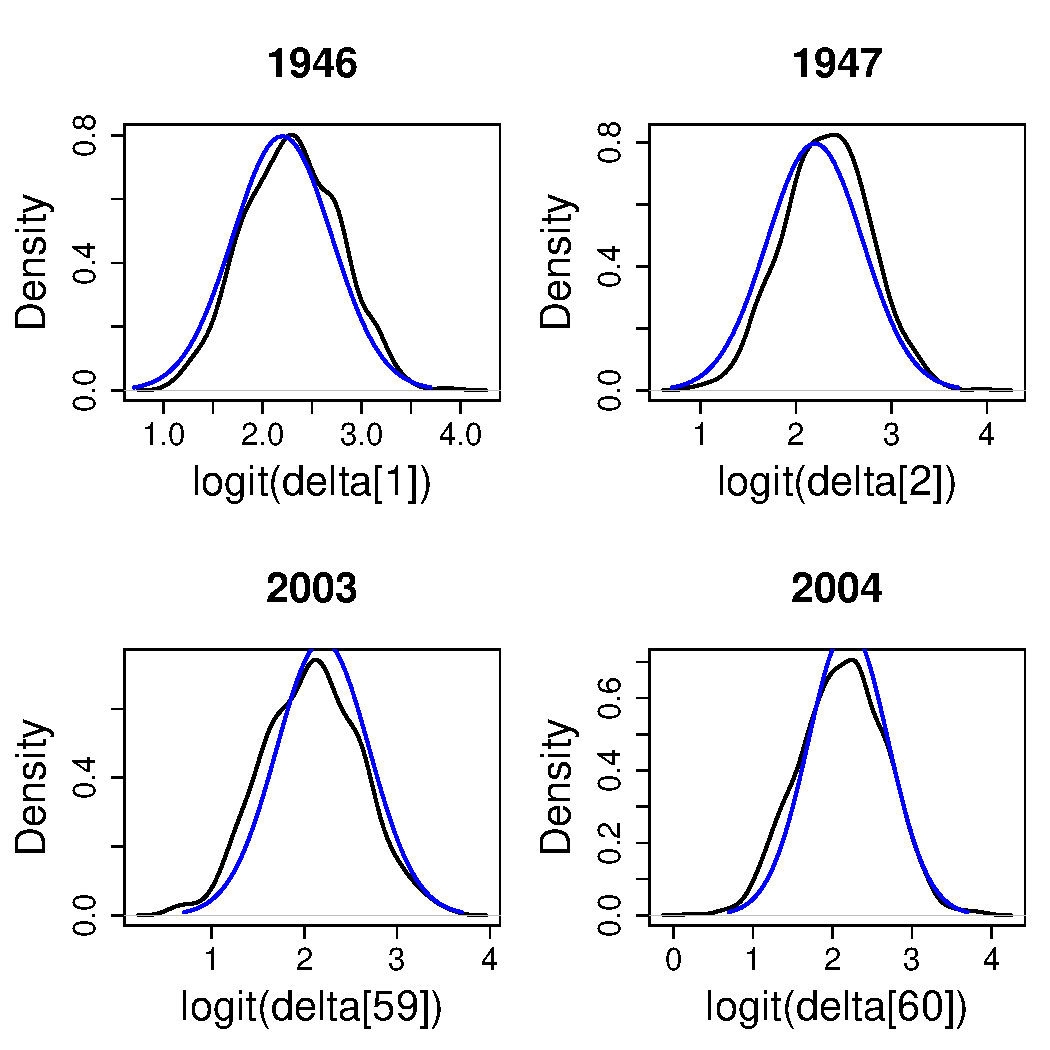
\includegraphics[height=7cm]{figure/Post_delta} 
\end{center}
\end{frame}

%-----------------------------------------------------------------------
%           Posterior kappa
%-----------------------------------------------------------------------

\begin{frame} 

\begin{center}
	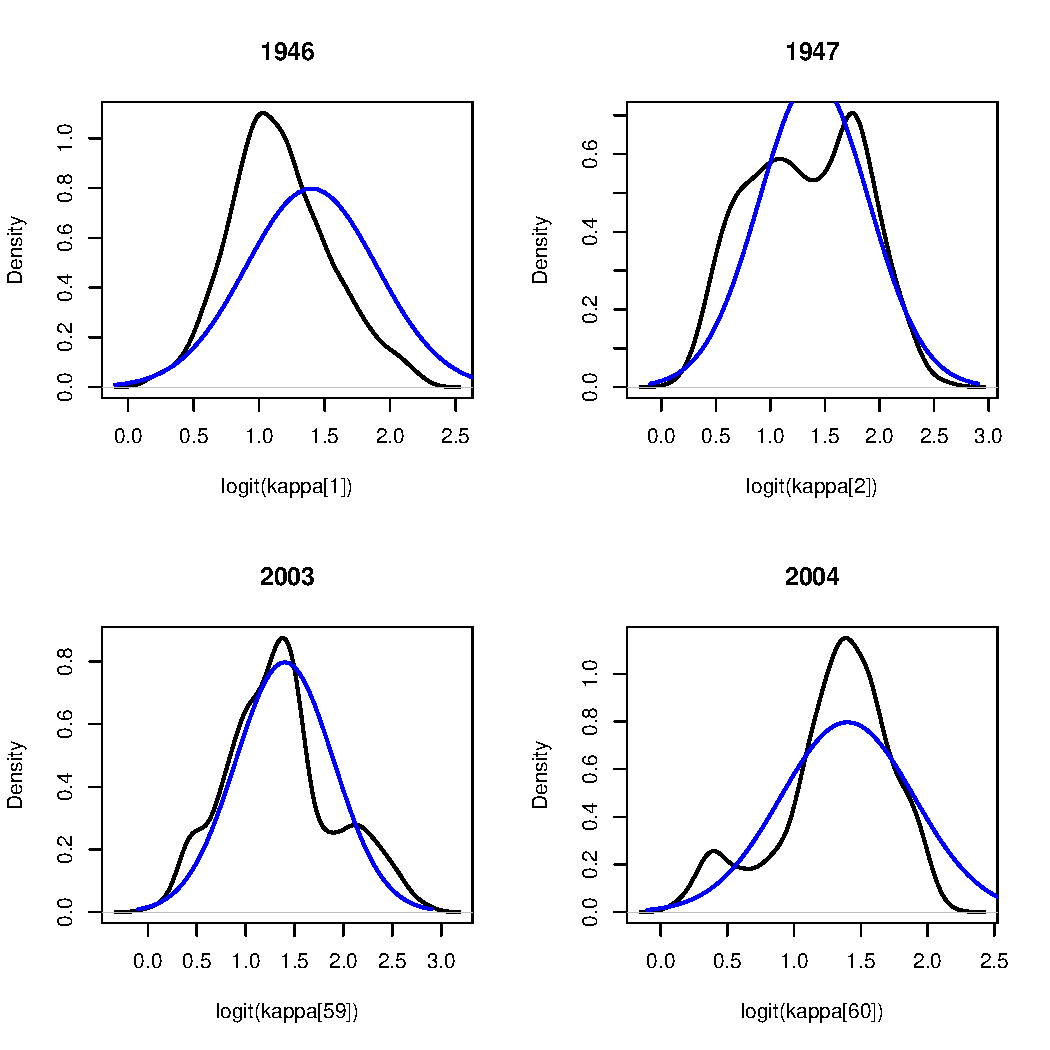
\includegraphics[height=7cm]{figure/Post_kappa} 
\end{center}
\end{frame}

%-----------------------------------------------------------------------
%           Posterior Eigenvalues
%-----------------------------------------------------------------------

\begin{frame} 

\begin{center}
	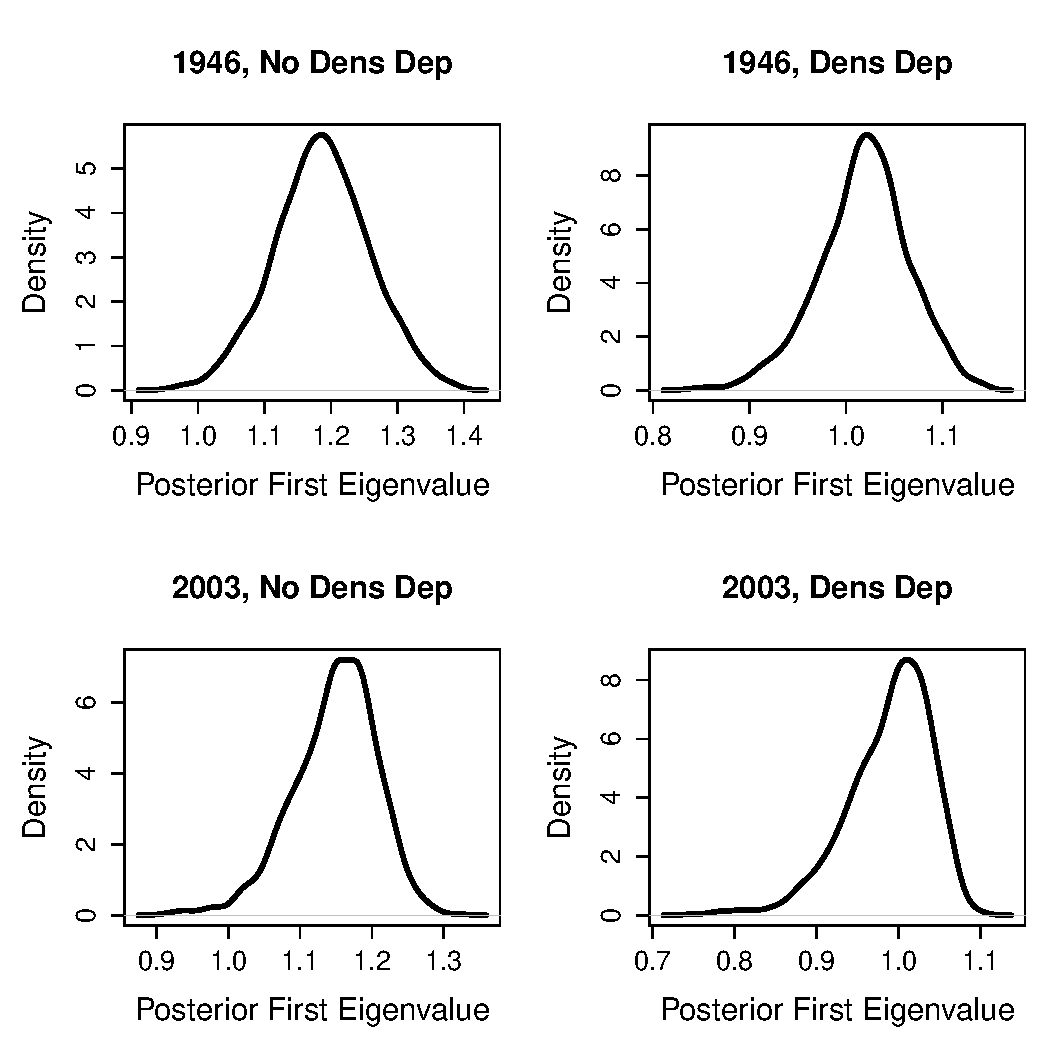
\includegraphics[height=7cm]{figure/Post_eigval} 
\end{center}
\end{frame}

%%%%%%%%%%%%%%%%%%%%%%%%%%%%%%%%%%%%%%%%%%%%%%%%%%%%%%%%%%%%%%%%%%%%%%%%%%%%%%%%%%
%%%%%%%%%%%%%%%%%%%%%%%%%%%%%%%%%%%%%%%%%%%%%%%%%%%%%%%%%%%%%%%%%%%%%%%%%%%%%%%%%%
%%%%%%%%%%%            %%%%%%%    %%%%%%%%  %%%%%%%       %%%%%%%%%%%%%%%%%%%%%%%%
%%%%%%%%%%%  %%%%%%%%%%%%%%%%%  %  %%%%%%%  %%%%%%%  %%%%  %%%%%%%%%%%%%%%%%%%%%%%
%%%%%%%%%%%  %%%%%%%%%%%%%%%%%  %%  %%%%%%  %%%%%%%  %%%%%%  %%%%%%%%%%%%%%%%%%%%%
%%%%%%%%%%%  %%%%%%%%%%%%%%%%%  %%%  %%%%%  %%%%%%%  %%%%%%%   %%%%%%%%%%%%%%%%%%%
%%%%%%%%%%%            %%%%%%%  %%%%  %%%%  %%%%%%%  %%%%%%%%  %%%%%%%%%%%%%%%%%%%
%%%%%%%%%%%  %%%%%%%%%%%%%%%%%  %%%%%  %%%  %%%%%%%  %%%%%%%   %%%%%%%%%%%%%%%%%%%
%%%%%%%%%%%  %%%%%%%%%%%%%%%%%  %%%%%%  %%  %%%%%%%  %%%%%%  %%%%%%%%%%%%%%%%%%%%%
%%%%%%%%%%%  %%%%%%%%%%%%%%%%%  %%%%%%%  %  %%%%%%%  %%%%  %%%%%%%%%%%%%%%%%%%%%%%
%%%%%%%%%%%            %%%%%%%  %%%%%%%%    %%%%%%%       %%%%%%%%%%%%%%%%%%%%%%%%
%%%%%%%%%%%%%%%%%%%%%%%%%%%%%%%%%%%%%%%%%%%%%%%%%%%%%%%%%%%%%%%%%%%%%%%%%%%%%%%%%%
%%%%%%%%%%%%%%%%%%%%%%%%%%%%%%%%%%%%%%%%%%%%%%%%%%%%%%%%%%%%%%%%%%%%%%%%%%%%%%%%%%


\end{document} 
